\chapter{Resultados y Análisis}

En este capítulo se describen ciertos pasos y funcionamientos de la solución en general, para esto se supone una habitación con un sensor de temperatura, un bombillo y una tira led, las cuales el usuario va a visualizar y gestionar desde la aplicación web. En la Figura \ref{fig:iot} está el esquema del sistema IoT.

\begin{figure}[H]
	\centering
	\caption[Esquema Solución SmartHouse.]{Esquema Solución SmartHouse. [Imagen Propia]}
	\label{fig:iot}
	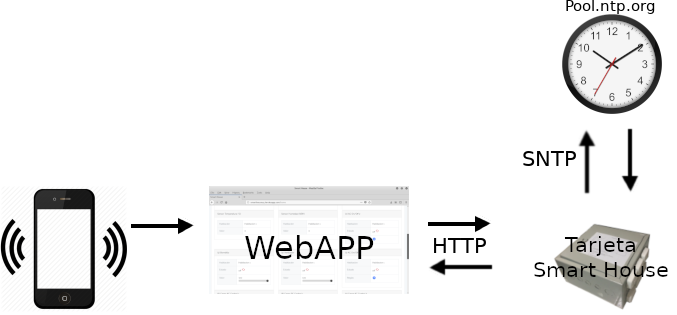
\includegraphics[width=0.7\linewidth]{Imagenes/IOT}
\end{figure}

\section{Software}

\subsection{Aplicación Web}

Para el usuario administrador algunas de sus vistas se observan en la Figura \ref{fig:r-adm}, las cuales permiten distinguir algunos usuarios creados y las otras opciones que tiene como visualizar, editar y eliminar. En la Figura \ref{fig:r-adm}\textbf{(a)} de la imagen se observan algunos dispositivos registrados en la aplicación web, el administrador puede editarlos pero no puede cambiar su estado o visualizar su valor, ya que esto es algo privado de cada dispositivo, además de que se presenta dependiendo de la habitación a la que pertenezca, en la Figura \ref{fig:r-adm}\textbf{(b)} se observan algunos usuarios creados y el mismo usuario administrador con sus datos y rol.

\begin{figure}[H]
	\centering
	\caption[Panel de Administrador.]{Panel de Administrador. [Imagen Propia]}
	\subfigure[Dispositivos]{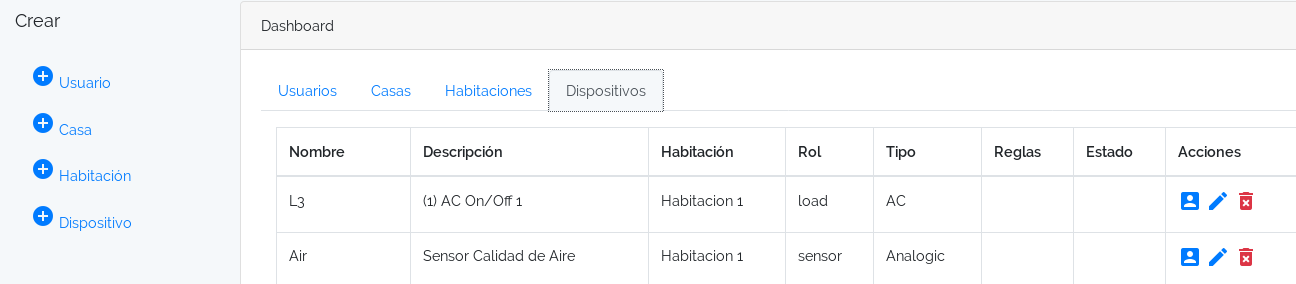
\includegraphics[width=\linewidth]{Imagenes/R_admA}}
	\subfigure[Usuarios]{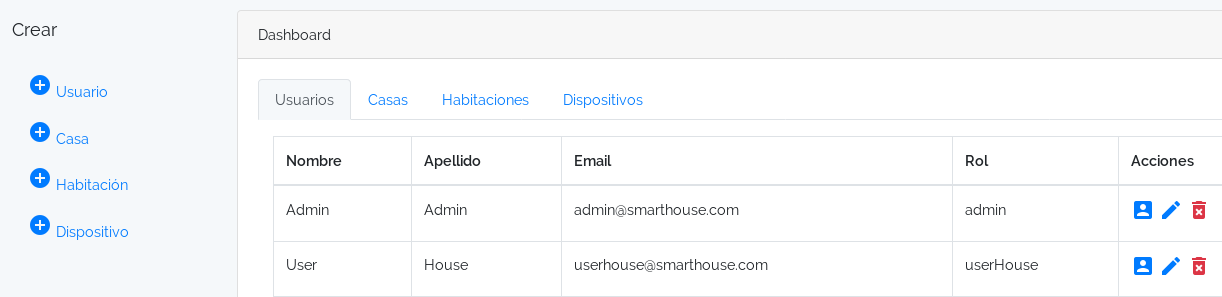
\includegraphics[width=\linewidth]{Imagenes/R_admB}}
	\label{fig:r-adm}
\end{figure}

Además en la Figura \ref{fig:r-room} se puede observar la habitación que se ha creado de prueba con sus correspondientes datos, nombre, descripción, usuarios y su token, el cual es muy importante para la seguridad de la comunicación entre el sistema embebido y la aplicación web, ya que este junto con el id de la habitación se precargan en la aplicación del sistema embebido, con el fin de que sea posible la correcta comunicación con la aplicación web a través de la red y que no genere errores con otros dispositivos registrados.

\begin{figure}[H]
	\centering
	\caption[Vista Habitación Usuario Administrador.]{Vista Habitación Usuario Administrador. [Imagen Propia]}
	\label{fig:r-room}
	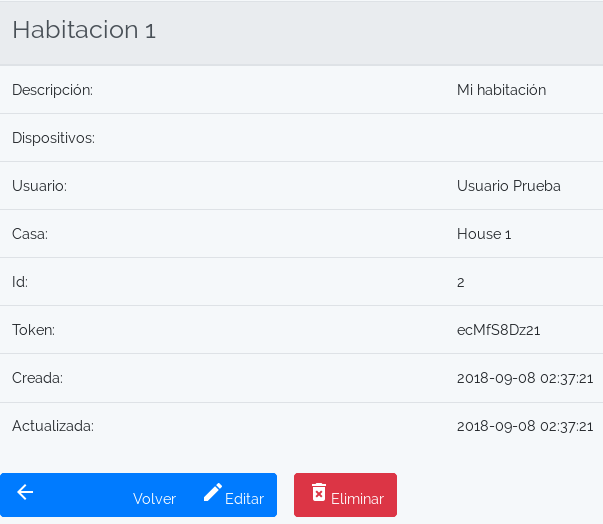
\includegraphics[width=0.45\linewidth]{Imagenes/R_room}
\end{figure}

Del mismo modo, el usuario habitación, se presenta un panel de control con todos los dispositivos presentes en su habitación, en este caso se puede observar en la Figura \ref{fig:r_app} que está el sensor de temperatura con su respectiva medida, también el bombillo y una tira LED apagada según la información que muestra la aplicación web. El sensor de temperatura arroja un valor de 23$^{\circ}$C según la imagen, el Bombillo está conectado en la salida (3) con el valor de potencia al mínima y se encuentra encendido y la tira LED está conectada a la salida (9) y apagada con el valor de potencia al máximo, es decir, al encender cualquiera de los dos dispositivos estos toman el valor que tienen de control, uno con la mínima potencia y el otro con el máximo. Para encender o apagar cualquiera de estos dispositivos se presiona en el botón rojo o verde según el caso en la parte de ``Estado'', para cambiar su valor se debe utilizar el deslizador propuesto en la fila ``Valor'', al usarlo se puede variar la potencia del dispositivo, también la tira LED tiene una fila adicional que muestra el estado de las reglas, en esta figura existe una regla de encendido configurada, por lo tanto a una hora provista se encenderá y en otra hora se apagará según se haya configurado, además se observa que todos los dispositivos pertenecen a la habitación con nombre ``Habitación 1''.

\begin{figure}[H]
	\centering
	\caption[Vista dispositivos habitación propuesta.]{Vista dispositivos habitación propuesta. [Imagen Propia]}
	\label{fig:r_app}
	\includegraphics[width=\linewidth]{Imagenes/R_app}
\end{figure}

Continuando con este usuario y la habitación modelo propuesta al inicio del capítulo, luego de que accede a la aplicación web e inicia sesión con los datos que ha registrado en el sistema, al ser un usuario de una habitación, este se encuentra con un panel de control como el de la Figura \ref{fig:views}\textbf{(c)}, compuesto por los items de la Figura \ref{fig:r_app}. Allí gestiona los dispositivos presentes en su habitación, así como también puede visualizar la temperatura que se ha sensado y encender o apagar los dispositivos conectados a la tarjeta, como se menciona anteriormente. Asimismo al realizar cualquier cambio en esta interfaz se refleja en el texto formato JSON que se envía a la tarjeta que se observa en la Figura \ref{fig:updateview} del capítulo anterior.\\

Cabe resaltar que cada sensor y salida se presentan en estas tarjetas y algunos con información diferente debido a su naturaleza, por ejemplo en la Figura \ref{fig:r_app1} se observa el sensor de lluvia con información de cuando detecto lluvia o dejo de detectar lluvia y también una salida DC para motor, como cuenta con inversión de giro el deslizador tiene valores entre -100 y 100, los valores negativas para que gire en un sentido y los valores positivos para el otro sentido.

\begin{figure}[H]
	\centering
	\caption[Vista dispositivos adicionales.]{Vista dispositivos adicionales. [Imagen Propia]}
	\label{fig:r_app1}
	\includegraphics[width=\linewidth]{Imagenes/R_app1}
\end{figure}

\subsubsection{Base de Datos}

La estructura de la base de datos se puede observar en la Figura \ref{fig:db}, aquí se observan los diferentes campos que posee cada tabla, además de las llaves y sus relaciones. Las relaciones presentes en esta estructura son de tipo 1:N, es decir, por ejemplo un usuario puede tener relacionadas N casas.\\

\begin{figure}[H]
	\centering
	\caption{Base de datos SmartHouse [Imagen Propia]}
	\label{fig:db}
	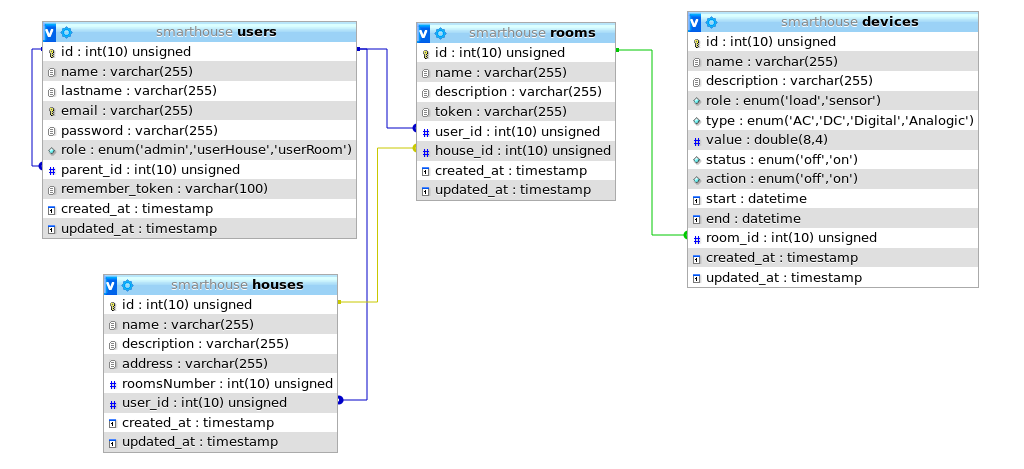
\includegraphics[width=0.75\linewidth]{Imagenes/DB}
\end{figure}

Esta sección donde se presentan todos los resultados en cuanto al software desarrollado presenta la mayoría de funciones implementadas en este, mostrando las diversas interfaces generadas en la aplicación, cumpliendo con los requisitos de permitir el monitoreo, control y la interacción del usuario con el dispositivo presente en su habitación, por medio de diferentes items que se han evidenciado en las figuras anteriores, permitiendo cambiar el estado de las salidas y asimismo visualizar los datos producidos por los sensores. También cabe resaltar que algunas salidas tienen la posibilidad de automatizarse a través de reglas, es decir, indicarle en que momento encender o apagar cierto dispositivo que se encuentre conectado a la tarjeta como se ha mencionado.\\

Las funcionalidades para el cambio de estado en las salidas se realizan con cuidado, generando diálogos de confirmación con el fin de que el usuario este seguro de la acción que realiza. Para ejercer control sobre la energía entrega a las cargas, se cuenta con un deslizador o slider que permite cambiar el porcentaje de esta, asimismo es significativo resaltar que todos los datos generados de la interacción del cliente con el programa, se almacenan en la base de datos enlazada a dicha aplicación permitiendo una gestión adecuada de estos. Los resultados obtenidos del diseño de este software cumplen con el objetivo a partir del cual se construye y también se tienen algunas funciones adicionales como los usuarios administradores de casa, esto asegurando la escalabilidad de la aplicación. \\

En cuanto a la protección de la aplicación se han mencionado los diferentes roles que se verifican por medio del middlware presente en esta solución, pero también cabe resaltar que con el objetivo de agregar seguridad a la transacción tarjeta-servidor se usa un token, el cual es único de cada habitación y se encuentra almacenado en la tarjeta y en el servidor, como se menciona anteriormente la aplicación al recibir la petición realiza esta verificación para proceder a contestar o simplemente ignorar la petición, de acuerdo con esto se esta ofreciendo un nivel de confiabilidad en dicha comunicación.\\

\subsection{Aplicación Sistema Embebido} 

Como se ha mencionado anteriormente, la aplicación se encuentra compuesta de tareas, en la Figura \ref{fig:tareas} se observa un bosquejo del trabajo de las diferentes tareas, tomando por función principal la encargada de gestionar la conexión a Wi-Fi y almacenar sus credenciales, dependiendo del estado de si están almacenadas o no, el sistema se comporta de una u otra forma. Si se encuentran credenciales guardadas en la tarjeta, el sistema se trata de conectar, si la conexión es exitosa comienza el proceso de actualización de la hora del sistema y también de las diferentes ordenes de la aplicación web. En cambio, si no existen credenciales el dispositivo inicia un servidor web local para que el usuario pueda proporcionarle esta información.\\

En cada caso se crean tareas diferentes, para el suceso de no existir credenciales únicamente se configura la tarea del servidor http local, y en la otra ocurrencia se lanzan todas la demás tareas encargadas de la escritura y lectura de datos, como se ha mencionado anteriormente en el capítulo de Desarrollo. Cabe resaltar que la tarjeta tiene disponible en promedio 160KB de memoria heap con el fin de poder realizar otras operaciones o implementar más funcionalidades en esta.\\

\begin{figure}[H]
	\centering
	\caption[Esquema de Tareas.]{Esquema de Tareas. [Imagen Propia]}
	\label{fig:tareas}
	
\includegraphics[width=0.7\linewidth]{Imagenes/tareas}
\end{figure}

Además de esto, se mide el promedio del tiempo en que se demora la ejecución de la tarea ``http\_get\_task'' en dos casos, cuando realiza la primera petición después de conectado a la red, es decir, cuánto se tarda realizando las peticiones necesarias, como obtener la hora y fecha de la red y realizar la petición a la aplicación web, obteniendo una duración media de aproximadamente de 2.7s, esta depende de la disponibilidad de los diferentes servidores en la web asimismo de la velocidad y el tráfico de la red, ya que la tarjeta espera hasta que obtiene dicha hora y luego continua con la petición HTTP también esperando que el servidor responda. El otro caso es el lapso que se demora la tarea en leer los datos de los sensores, enviar la petición HTTP al servidor, recibirlos y enviarlos a los diversos actuadores, este periodo es de 1s en promedio, para conocer el dato se tomaron un total de 3056 muestras.

\subsubsection{Conexión a Internet vía Wi-Fi}

Los sistemas IoT deben estar conectados siempre a Internet, por tal motivo se debe brindar una forma para conectar al sistema a este, en base a esto, se cuenta con un servidor local en la tarjeta que facilita este proceso, como se ha mencionado el módulo del ESP32 funciona como Punto de Acceso (AP) y como Cliente o Estación (STA) al mismo tiempo, aprovechando esta capacidad se usa el servidor local que se encuentra encargado de gestionar la conexión de la tarjeta vía Wi-Fi como se observa en la Figura \ref{fig:conexion}.\\

\begin{figure}[H]
	\centering
	\caption[Conexión a Internet vía Wi-Fi ESP32.]{Conexión a Internet vía Wi-Fi ESP32.  [Imagen Propia]}
	\label{fig:conexion}
	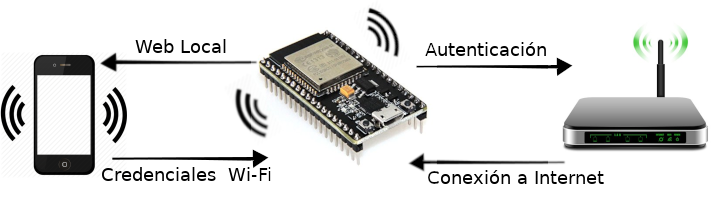
\includegraphics[width=0.9\linewidth]{Imagenes/conexion}
\end{figure}

De este modo, en la Figura \ref{fig:wifi} están algunas páginas del servidor local. En la Figura \ref{fig:wifi}\textbf{(a)} es posible observar la lista de las diferentes redes al alcance de la tarjeta, basta con seleccionar una red e ingresar sus credenciales para conectarse. En la Figura \ref{fig:wifi}\textbf{(b)} se observan los detalles de la conexión actual y también la opción de desconectarse. Su funcionamiento es muy intuitivo, se selecciona la red a la que se desea conectar la tarjeta, se ingresan sus credenciales y posteriormente el dispositivo verifica si la conexión fue exitosa o no; si lo es, la tarjeta esta lista para su funcionamiento, no obstante, se debe reiniciar para que solo quede funcionando como STA y no en el modo dual, además de esto si las credenciales de la red cambian, se incluye un botón para el borrado de estas, con el fin de que se puede configurar de nuevo el enlace con la red Wi-Fi.

\begin{figure}[H]
	\centering
	\caption[Aplicación Conexión a Wi-Fi.]{Aplicación Conexión a Wi-Fi. [Imagen Propia]}
	\label{fig:wifi}
	\subfigure[Lista de Redes]{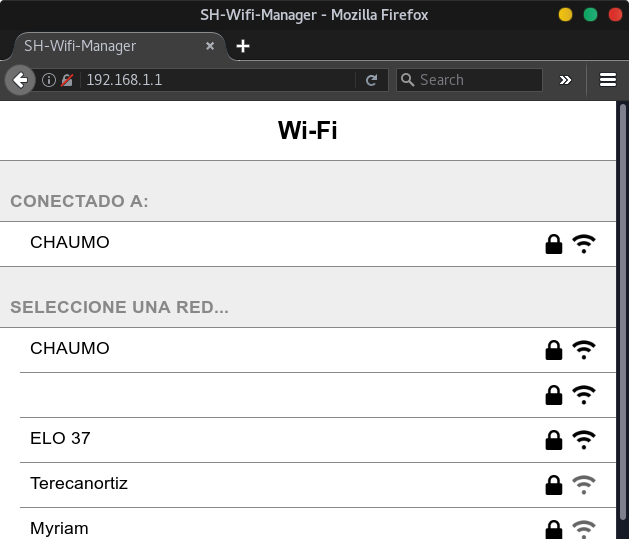
\includegraphics[width=0.45\linewidth]{Imagenes/w_status}
		\label{fig:red}}
	\subfigure[Datos de Conexión]{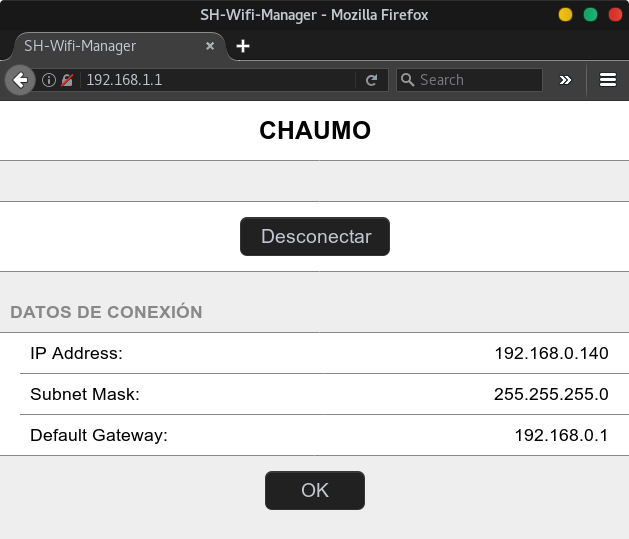
\includegraphics[width=0.45\linewidth]{Imagenes/w_red}
		\label{fig:opt}}
\end{figure}

\subsubsection{Escritura de Datos en la Aplicación Web}

Los datos que lee la tarjeta provienen de los diferentes sensores que tiene conectados según se ha mencionado, se usan diversos tipos, de estado para sensar la presencia, de calidad de aire entre otros presentes en esta. Para la escritura de los datos en la aplicación del ESP32 se desarrollaron varias tareas encargadas de leerlos y enviarlos a una tarea central como se menciona en el capítulo anterior. Los datos que están enviando contienen el id del dispositivo y la medida que lee en ese momento, estos se envían en forma de texto en formato JSON, de este modo, la tarea central los gestiona y envía a la aplicación con el mismo formato, organizandolos en la petición HTTP tipo GET que realiza, así la url que la tarjeta solicita, incluyendo el JSON de cada sensor, se observa en la Figura \ref{fig:json}, de esta manera, en la url se encuentra el dominio del servidor, y la dirección que contiene el id y token de la habitación, por último se halla la información del sensor en formato JSON, que se compone por el id y el valor de este. La aplicación ya se encarga de almacenarlos y mostrarlos al usuario.\\

\begin{figure}[H]
	\centering
	\caption[URL de la petición HTTP.]{URL de la petición HTTP. [Imagen Propia]}
	\label{fig:json}
	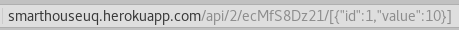
\includegraphics[width=0.7\linewidth]{Imagenes/JSON}
\end{figure}


\subsubsection{Lectura de Datos de Internet}

Para la configuración y comparación de las reglas que suministra el usuario a el dispositivo que desee controlar, es necesario contar con la hora actual y que se siga actualizando localmente gracias al RTC que posee internamente el ESP32, así, al inicio de la aplicación, se sincroniza y almacena la hora actual de la red, por medio del protocolo SNTP. Estas reglas actúan en cuanto a que encienda o apague un dispositivo en un instante dado, después de obtener este dato la ejecución programa continua con normalidad para realizar las diferentes peticiones a la aplicación web.\\

La interacción del usuario se da con la aplicación web mencionada anteriormente, de este modo la tarjeta siempre se debe actualizar, para esto, cuando la tarjeta envía los datos de los sensores, la aplicación responde con datos de cabecera HTTP y además la información de los dispositivos que controla la tarjeta, esta los recibe en una cadena texto en formato JSON como se observa en la Figura \ref{fig:httprqstesp}, los procesa y los dirige a las tareas pertinentes ya sea para encender o apagar algún dispositivo conectado a la tarjeta, también remite las reglas que el usuario ha definido.\\

\begin{figure}[H]
	\centering
	\caption[Respuesta del la APP Web a la Tarjeta.]{Respuesta del la APP Web a la Tarjeta.  [Imagen Propia]}
	\label{fig:httprqstesp}
	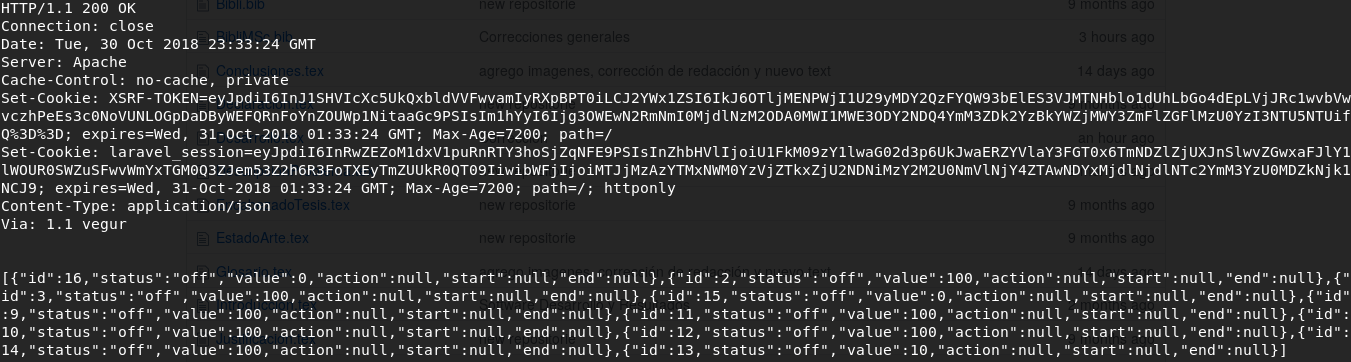
\includegraphics[width=0.8\linewidth]{Imagenes/HTTPRqstesp}
\end{figure}

Según lo presentado en esta sección, la tarjeta cuenta con funcionalidades para conectarse con Internet por medio de wi-fi, toda la configuración del cómo hacerlo la realiza el usuario mediante las herramientas ofrecidas por el programador, es decir, el servidor local. Durante el desarrollo de este programa se comprenden diferentes funciones que provee un RTOS, de manera que es viable haber desarrollado esta aplicación basado en este sistema operativo.\\

Analizando los tiempos de resolución de la petición http, siempre se tiene una media de 1s el cual es un tiempo de respuesta aceptable dadas todas las funcionalidades provistas en el programa, aunque este tiempo varia, ya que se usa el puerto serie para observar estos resultados, esta comunicación agrega también tiempo al procesamiento, así que es un aproximado, asimismo interfiere la velocidad en la conexión a Internet y la señal de recepción de Wi-Fi.\\

Por los resultados expuestos, el programa esta realizando correctamente las funciones necesarias para el monitoreo y control del ambiente de instalación, es decir, se cumple con los alcances provistos y además aún existen recursos de procesamiento para agregar nuevas funcionalidades o mejorar el desempeño.\\

\section{Hardware}

De acuerdo con los circuitos diseñados en la Sección \ref{sec:hw} donde se propone el desarrollo de hardware de la solución IoT, en la Figura \ref{fig:tarjeta} se observan las diferentes tarjetas ya ensambladas en una caja eléctrica para probar el funcionamiento del prototipo. Las salidas y entradas están distribuidas según lo propuesto, para las salidas AC se usan toma corrientes para conectar allí los diversos dispositivos, para las salidas DC se utilizan conectores hembra tipo banana para facilitar la conexión de estos dispositivos. El esquemático de los diferentes circuitos presentes en las dos tarjetas desarrolladas se ha mostrado en el capítulo anterior en la sección de desarrollo de hardware.\\

\begin{figure}[H]
	\centering
	\caption[Tarjeta SmartHouse.]{Tarjeta SmartHouse. [Imagen Propia]}
	\label{fig:tarjeta}
	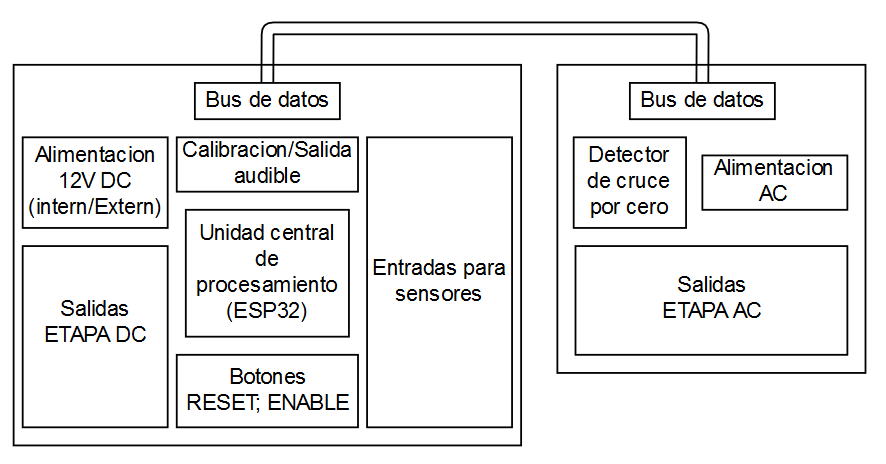
\includegraphics[width=0.6\linewidth]{Imagenes/Tarjeta.jpg}
\end{figure}

La distribución de las diferentes salidas que posee la tarjeta se organizó en pegatinas y se colocaron sobre la caja eléctrica. La Figura \ref{fig:labels} muestra esta información, tanto para la parte interna como externa de la caja.\\

\begin{figure}
	\centering
	\caption[Descripción caja eléctrica tarjeta SmartHouse.]{Descripción caja eléctrica tarjeta SmartHouse. [Imagen Propia]}
	\label{fig:labels}
	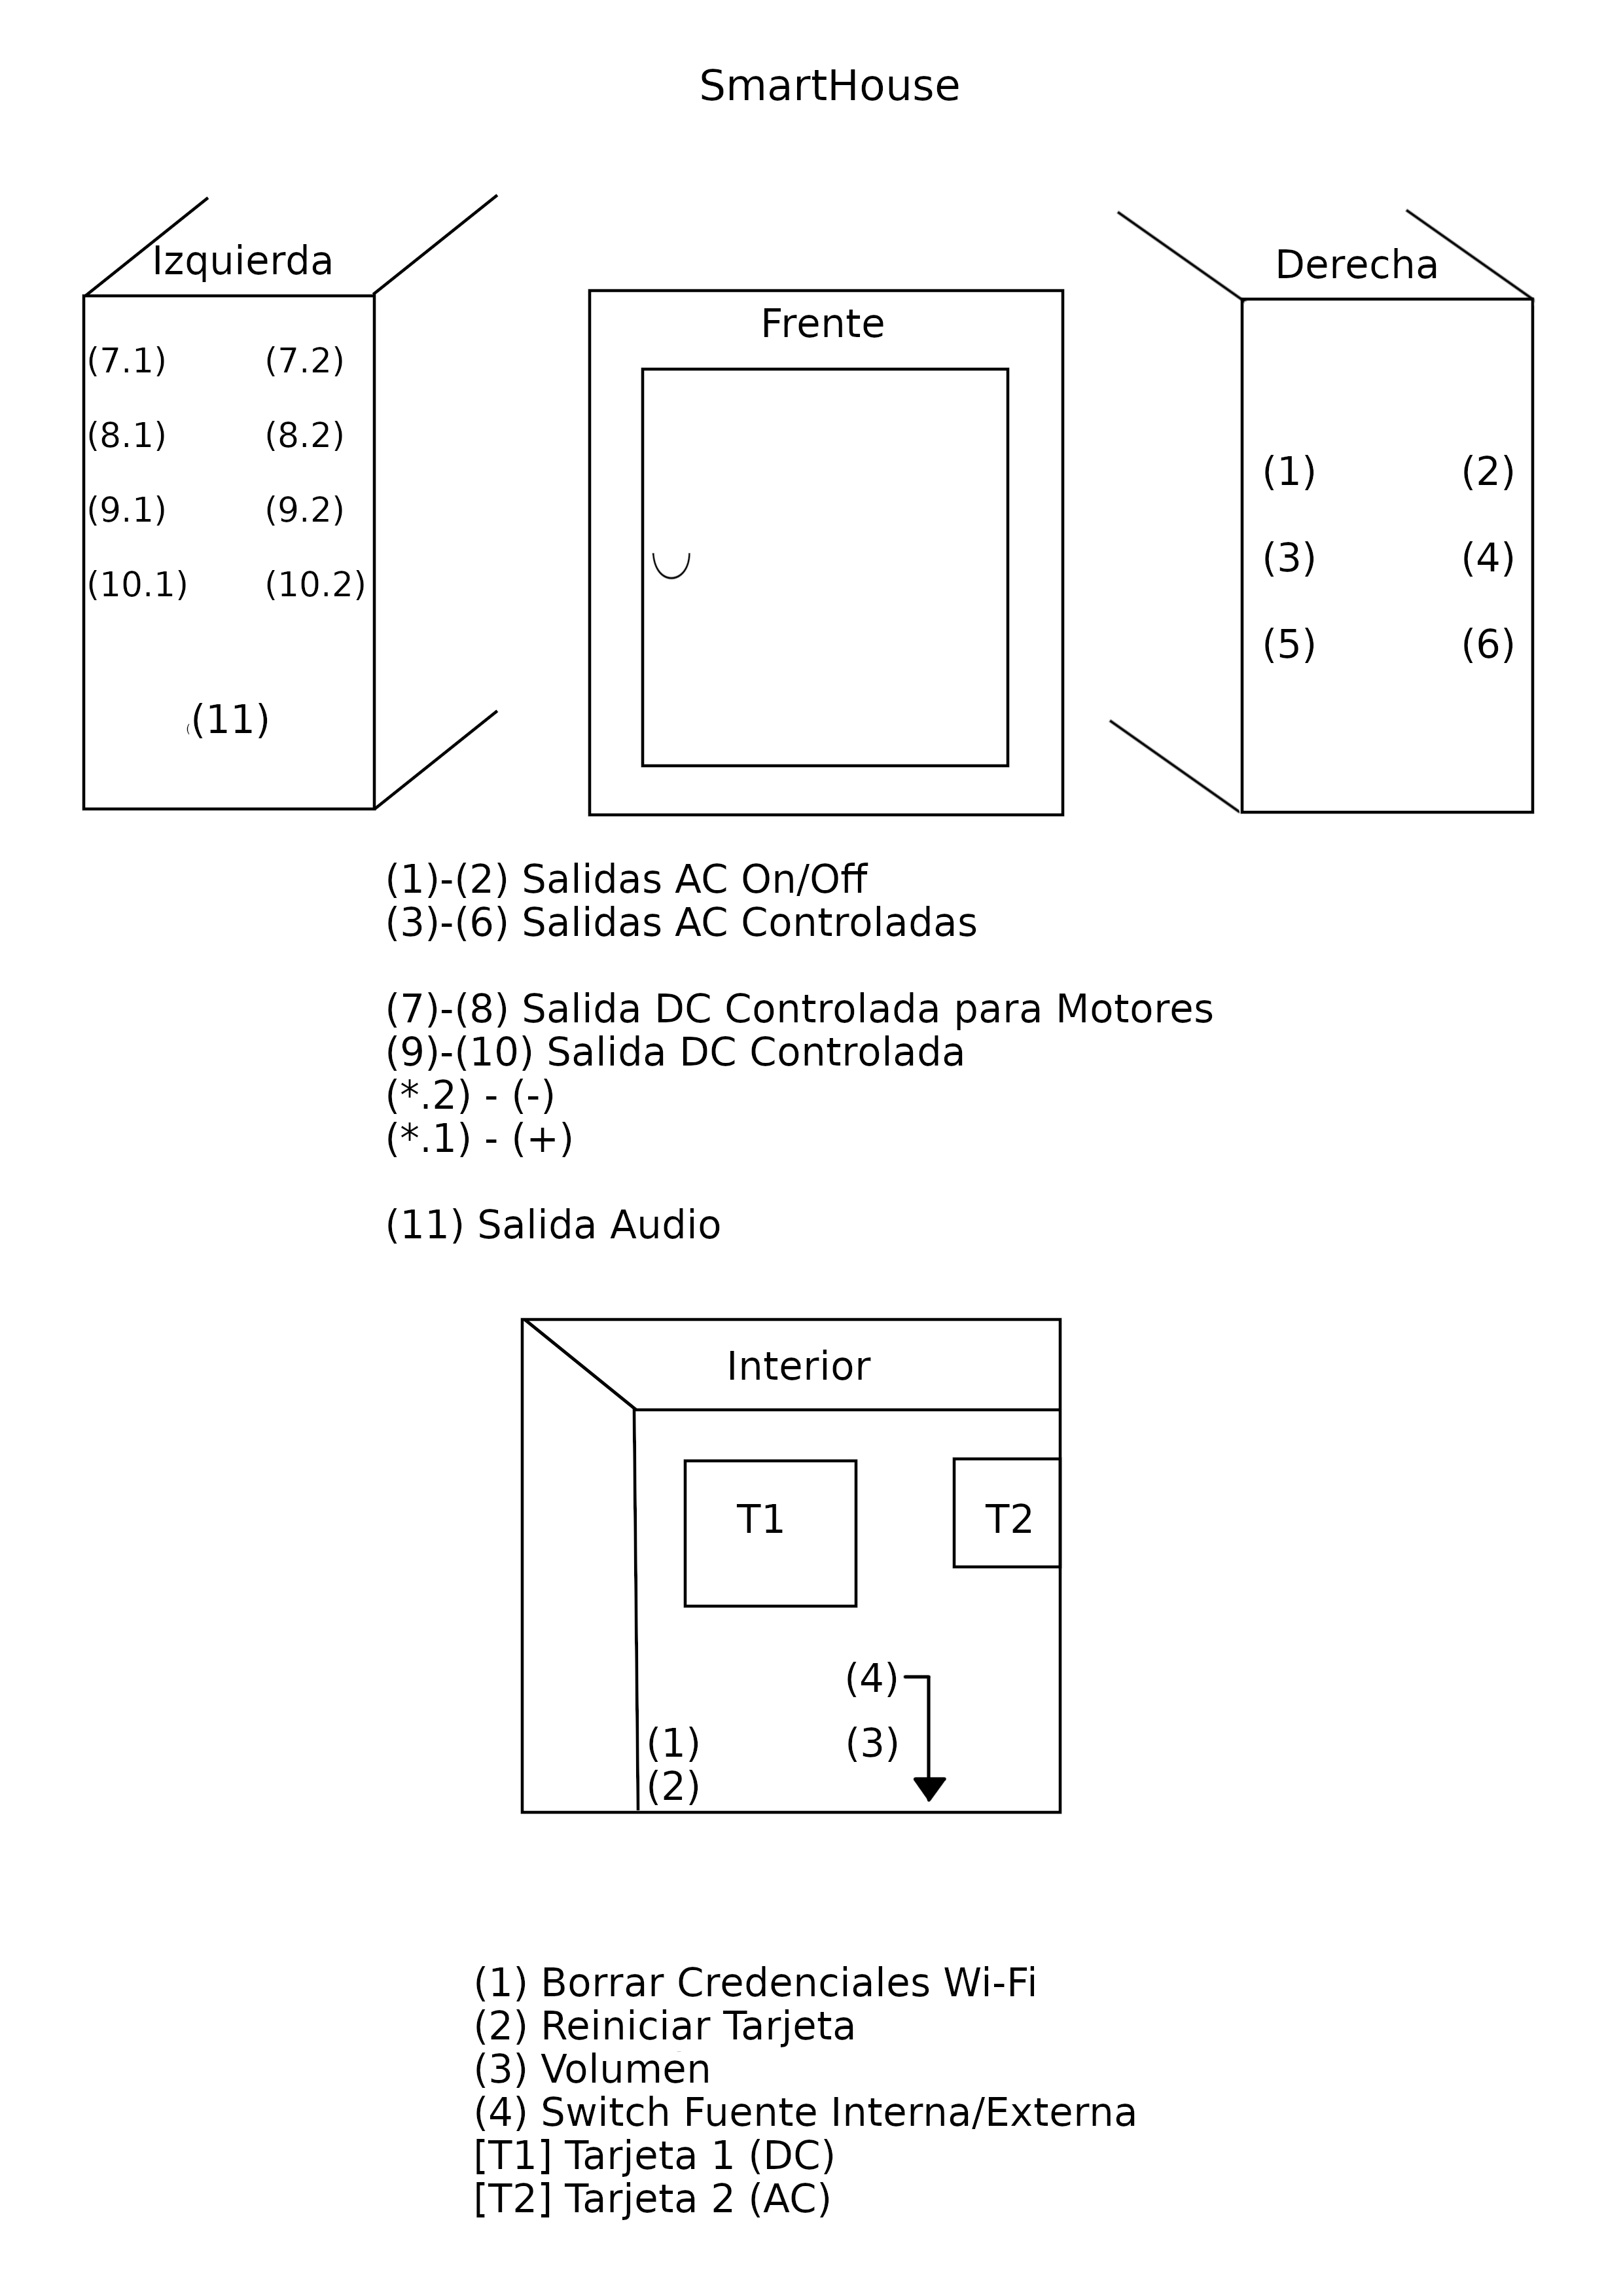
\includegraphics[width=0.7\linewidth]{Imagenes/labels}
\end{figure}

Conforme a lo mencionado anteriormente, el sistema se ha probado con cargas AC como bombillos LED entre 7W y 20W, de filamento de 100W, probando funcionalidades como el control de potencia AC por ángulo de fase, obteniendo los resultados esperados, según se observa en la Figura \ref{fig:ACc} donde la carga tiene el 100\% de la potencia. El voltaje de alimentación viene dado por la red eléctrica, la tarjeta simplemente conmuta el estado de la alimentación o controla la potencia entregada.\\

\begin{figure}[H]
	\centering
	\caption[Control de potencia AC por ángulo de fase.]{Control de potencia AC por ángulo de fase. [Imagen Propia]}
	\label{fig:ACc}
	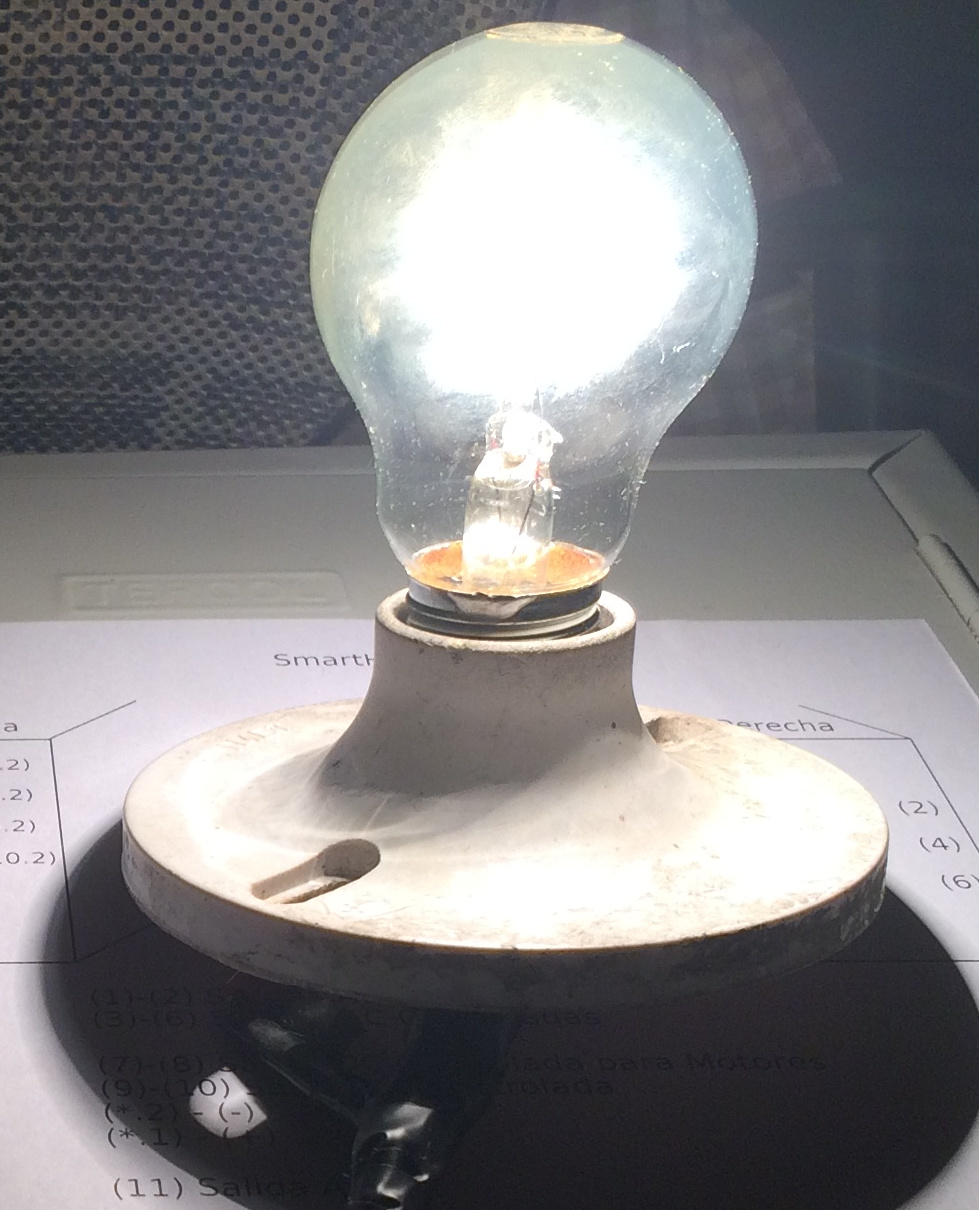
\includegraphics[width=0.3\linewidth]{Imagenes/AC1}
\end{figure}

Para las salidas DC se realizan pruebas con un motor DC de 1W, además de una tira LED de 1W, la cual se le varia la energía entrega, como se observa en la Figura \ref{fig:DCc} la carga tiene el 100\% de la energía. Estas cargas se alimentan con 12VDC directamente desde la fuente o convertidor AC-DC, los circuitos que se implementan simplemente conmutan el estado de encendido/apagado o por medio de PWM variar la energía entregada.\\

\begin{figure}[H]
	\centering
	\caption[Control de cargas DC.]{Control de cargas DC. [Imagen Propia]}
	\label{fig:DCc}
	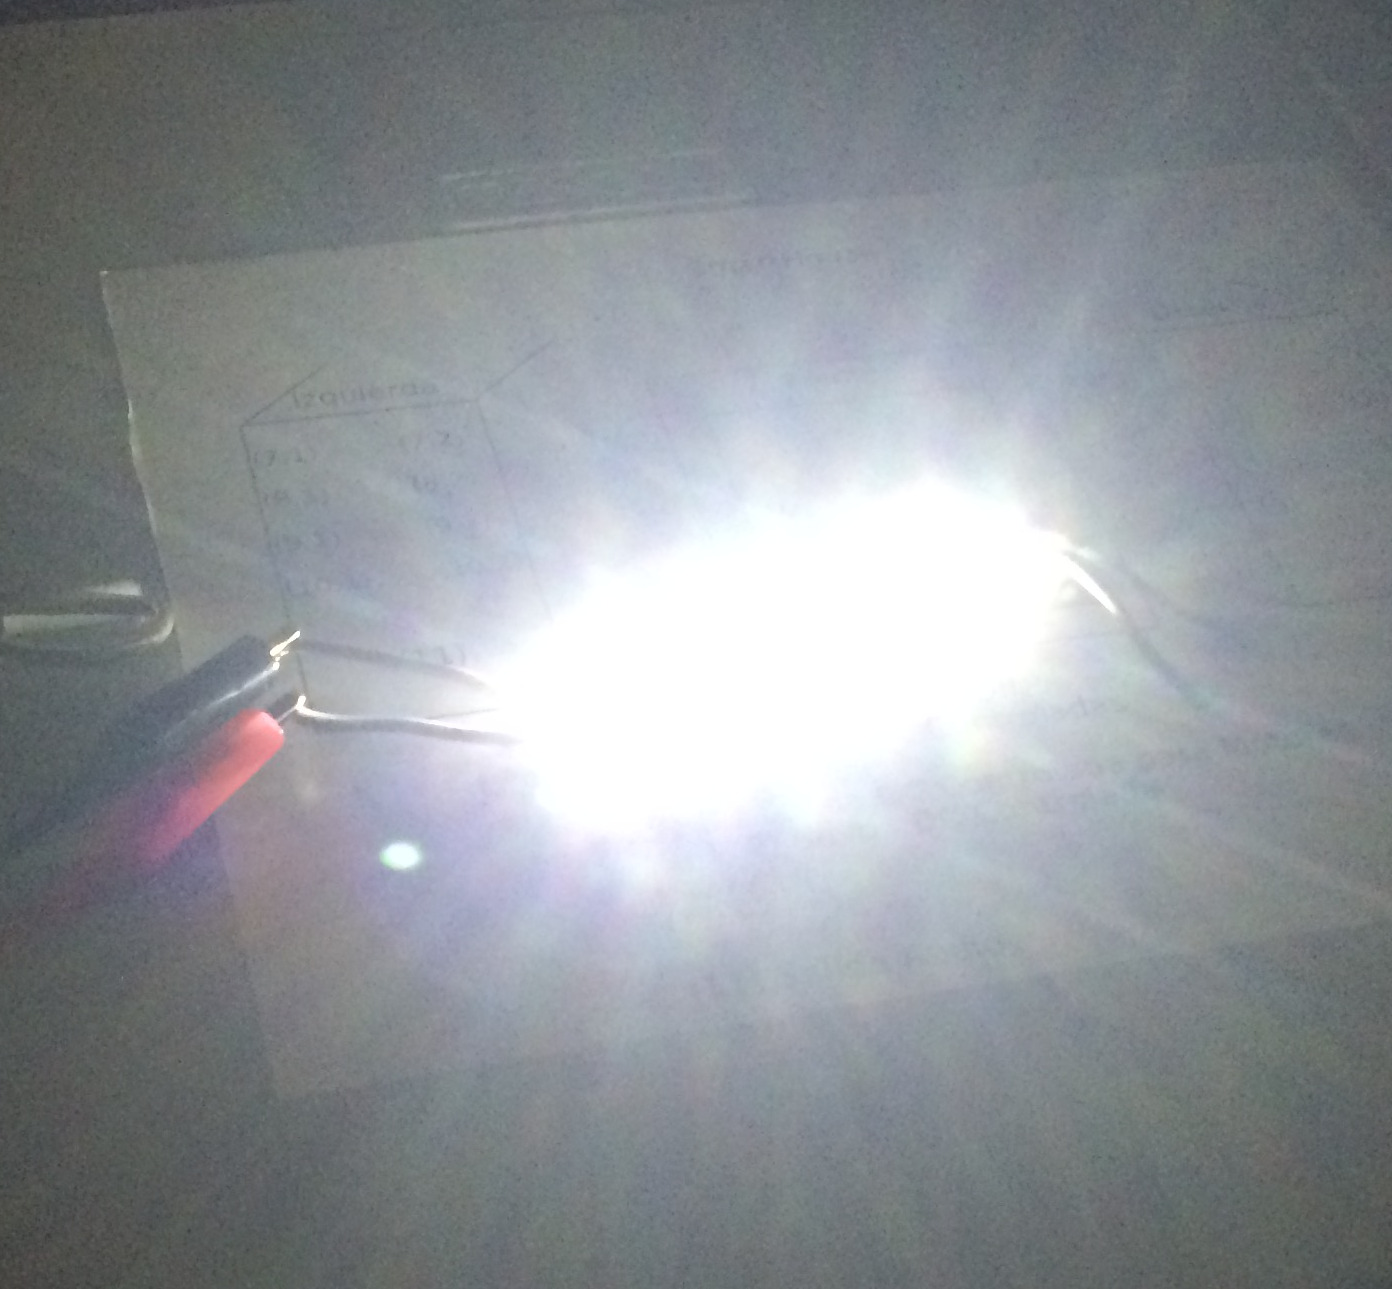
\includegraphics[width=0.5\linewidth]{Imagenes/DC1}
\end{figure}

En esta sección se evidencia tanto el hardware implementado, como su correcto funcionamiento de acuerdo con los requisitos propuestos, proporcionando las diferentes funcionalidades para que la aplicación realice la gestión adecuada, es decir, controlar las salidas y recibir la información de los entradas. Se han construido diferentes circuitos, los cuales por medio del programa gestiona los diferentes dispositivos conectados a este.\\

Se observa que el hardware quedo dividido en dos tarjetas, esto para facilitar la construcción y distribución de los diferentes elementos utilizados, si se usan componentes superficiales y se aumentan las capas de la tarjeta es posible reducir el tamaño y hasta integrarlas en una sola board. En la construcción de estas tarjetas se comprende diferentes funcionamientos en cuanto a los triac y los transistores mosfet, reforzando conocimientos que se habían adquirido.\\

\section{Prueba Beta Cerrada}

Esta prueba se desarrolla en el entorno del cliente o usuario, arrojando resultados sobre las funcionalidades provistas para el software, además de dar la aceptación por parte del cliente si el producto funciona de manera adecuada o esperada \cite{PB}. Con el fin de realizar dicha verificación se analizan los objetivos a cumplir y los alcances, por lo tanto se separan los casos de prueba con el propósito de formular las preguntas que deben contestar las personas.\\

En general se ha propuesto el desarrollo de una solución IoT, con alcances como controlar cargas AC o DC y visualizar el estado del entorno de aplicación por medio de la página web desarrollada, además de que esta aplicación web sea fácil de usar para el usuario, por este motivo se presentan los diferentes casos de prueba a realizar y se mencionan a continuación; las preguntas formuladas para estos se encuentran en el Anexo \ref{AnexoB}.

\paragraph{Prueba de conectividad de la tarjeta:} La persona que participa en esta prueba debe realizar los primeros pasos para conectar la tarjeta con internet como se expone más adelante en resultados y se explica en Anexos en el manual de usuario.\\

De acuerdo con esto se califica la forma en que el cliente realiza este procedimiento, con la finalidad de analizar si es adecuada la manera en que se conecta la tarjeta SmartHouse a Internet por medio de Wi-Fi y también como reiniciar la conexión de la tarjeta para configurar nuevamente la red a la que se va a conectar. Las preguntas que califican esta funcionalidad se mencionan a continuación:\\

\begin{itemize}
\item El método para conectar la tarjeta a Internet por medio de Wi-Fi es sencillo de realizar.
\item La interfaz para seleccionar la red e ingresar las credenciales es fácil de utilizar.
\item En caso del cambio de nombre o contraseña de su red Wi-Fi, es fácil volver a configurar la tarjeta para que esta se conecte de nuevo.
\end{itemize}

\paragraph{Prueba de la Aplicación Web:} Evalúa el inicio de sesión, el monitoreo y control de todos los dispositivos que se encuentra conectados en tarjeta SmartHouse, además de las funcionalidades que posee el sistema en general.\\

Para esta prueba se deben realizar diferentes procedimientos, como iniciar sesión en la aplicación, encender o apagar un dispositivo, visualizar los datos de los sensores y configurar las reglas para los dispositivos. Las preguntas presentadas a continuación califican estos aspectos y funcionalidades:\\

\begin{itemize}
	\item El inicio de sesión en la pagina web es claro.
	\item En la aplicación web, los datos de los sensores y estados de las salidas se presentan de una manera clara y entendible.
	\item Encender o apagar un dispositivo o salida es sencillo y se presenta de forma clara.
	\item El tiempo de respuesta después de encender o apagar un dispositivo desde la aplicación es bueno.
	\item Las reglas para los dispositivos o salidas son fáciles de configurar y eliminar.
	\item La aplicación web es fácil de usar.
\end{itemize}

Para la prueba beta se escoge un grupo de personas, las cuales interactuan directamente con la aplicación web y el prototipo de la tarjeta SmartHouse, se detallan los diferentes items a evaluar mencionados anteriormente, como el ingreso a la aplicación, visualización de los datos almacenados en esta y el control de los dispositivos.\\

Así, para evaluar estas características se toman las preguntas formuladas, que se califican de acuerdo con una escala tipo likert \cite{lik} de uno a cinco en la cual, cinco es la calificación máxima y uno la mínima. Estas se formulan para evidenciar la postura del cliente en cuanto a las funcionalidades de la aplicación, conforme a esto la encuesta que se diseña esta presente en el Anexo \ref{AnexoB}.\\

Al ser una prueba beta cerrada el desarrollador escoge un número de personas determinadas con distintas características, por este motivo se realiza a quince personas, entre los cuales algunos son estudiantes de ingeniería electrónica, estudiantes de otras carreras, profesionales y personas ajenas a este tipo de escenarios, los resultados de la prueba se consignan en la Tabla \ref{table:enc} y también en el Anexo \ref{AnexoC} en forma digital, realizando el promedio de cada pregunta y presentando un resultado total, además en los anexos se encuentra el documento que cada persona respondió.\\

\begin{table}[H]
	\begin{center}
		\caption{Resultados por pregunta.}
		\label{table:enc}
		\begin{tabular}{|c|c|}
			\hline 
			\textbf{Número de la Pregunta} & \textbf{Promedio} \\ 
			\hline 
			1 & 4.5\\ 
			\hline 
			2 & 4.8\\ 
			\hline 
			3 & 4.5\\ 
			\hline 
			4 & 5.0\\ 
			\hline 
			5 & 4.9\\ 
			\hline 
			6 & 4.9\\ 
			\hline 
			7 & 4.3\\ 
			\hline 
			8 & 4.3\\ 
			\hline 
			9 & 4.8\\ 
			\hline 
			\textbf{Total} & \textbf{4.7}\\ 
			\hline 
		\end{tabular} 
	\end{center}
\end{table}

De acuerdo con los resultados es necesario analizar cada pregunta individualmente y también en su totalidad, así se pueden identificar las funciones a mejorar en el sistema. Con respecto al método de conexión de la tarjeta a Internet se obtiene un promedio de 4.5, indicando que los pasos que se deben cumplir para realizarlo están claros pero aún falta mejorarlos para su total comprensión, ya que la mayoría de personas encuestadas manifestó esta opinión. Esto sucede por la poca interacción que el usuario normalmente tiene con la configuración de dispositivos, de este modo se puede brindar ayuda telefónica o del servicio técnico en momento de la instalación.\\

Asimismo, la interfaz que se provee para realizar la conexión del sistema a la red Wi-Fi obtiene una calificación de 4.8. Las personas encuestadas exponen que es de fácil uso pero faltan explicaciones en cuanto al momento de ingresar a esta. Se puede implementar también un DNS con la finalidad de que los usuarios no ingresen una dirección IP al navegador sino que escriban un nombre de dominio.\\

Además, em caso de que la red Wi-Fi cambie sus credenciales se provee un pulsador para eliminar estas, esta funcionalidad recibe una calificación de 4.5, algunos de los comentarios realizados sugieren el cambio de posición de este botón, ya que no se visualiza fácilmente y de una explicación un poco más detallada de esto, si es posible tener acompañamiento del personal técnico.\\

Después, al ingresar a la pagina web se presentan de manera clara los botones en la interfaz, es decir, el inicio de sesión obtiene una calificación de 5.0 lo que indica que para el usuario es fácil realizar dichas acciones, ya que los usuarios normalmente están muy familiarizados con estas, por ejemplo, cuando ingresan a redes sociales.\\

En cuanto a cómo se presenta la información de los diferentes dispositivos en el panel de control se obtiene 4.9, es decir, estos datos se presentan de manera clara y entendible para el usuario pero falta añadir un poco de explicación con el fin de que este se familiarice más con la interfaz propuesta.\\

Luego, en la parte de gestionar las salidas desde la web la calificación fue de 4.9, por lo tanto la manera en que se encienden, apagan y se controlan los diferentes dispositivos es claro, pero por ejemplo, por el tiempo de recarga automática de la página a veces es necesario cierta rapidez para cambiar alguna característica. Por tal motivo se modifica este lapso de 10s a 20s, de acuerdo con las observaciones realizadas.\\

Por otra parte, el tiempo de respuesta después de gestionar un dispositivo en la aplicación obtuvo 4.3, es una calificación baja respecto a las demás, este resultado depende de diversas circunstancias que se presenten durante la realización de la instrucción y todo lo que esto acarrea, desde el momento en que el usuario realiza la acción, es decir, que no coincida con la actualización automática de la pagina, la rapidez del navegador que posee el dispositivo desde el que realizan la actividad, entre otros factores también propios del programa, por ejemplo, el tiempo que la tarea esta suspendida o el lapso de ejecución de la instrucciones.\\

Respecto a la activación de las reglas para los dispositivos la calificación es de 4.3, ya que no es muy claro para el usuario qué es una regla dentro de la aplicación, además de que no están disponibles en todas las salidas por este motivo se puede mejorar la interfaz con el fin de definirlas de una mejor manera, asimismo hacerla más interactiva e intuitiva con el cliente.\\

Además, en una escenario general la facilidad de uso de la aplicación web recibe 4.8 como calificación, es decir que cumple con las expectativas, pero requiere agregar ciertos cambios para que sea más fácil de usar la primera vez que el cliente tiene contacto con esta. En este punto se resaltan observaciones ya mencionadas como el tiempo de actualización automática de la aplicación y la distribución del panel de control.\\ 

En resumen, la aplicación recibe una calificación de 4.7, por lo tanto se puede decir que las funcionalidades requeridas están programadas de una manera adecuada y simple para que el usuario disponga de ellas, pero es posible mejorarlas con el objetivo de que sean mucho más intuitivas para el usuario y que no se le presenten dudas al momento de usarla. Conforme a las observaciones obtenidas durante la prueba se han modificado algunas partes del sistema, que no tienen un impacto significativo sobre los objetivos ni alcances propuesto en este trabajo.\\